%!TEX root=../main.tex
\chapter{Climbing Mont Blanc Improvements}
\label{ch:improvements}

In this chapter it is assumed that a web interface follows the \gls{mvc} pattern. As briefly mentioned in sub-section \ref{subsec:cmb-arch-frontend}, Angular structures the HTML and Javascript code according to the \gls{mvc} pattern, and the reader should have the abstraction in mind when reading about browser or frontend implementations.

\section{Dynamic Update}
The frontend view changes when a user performes actions against the frontend models as mentioned in sub-section \ref{subsec:cmb-arch-frontend}. However, the frontend view presented to a given user does not update automatically as other users interract and changes their data models, as models is stored locally in each of the user's browser. If the updated model contains data that should be known\footnote{Hereby known as \textit{shared data}.} to all users, the users does not get notified about the model changes dynamically and views may therefore display out of date information. Figure \ref{fig:update-problem} shows an example of the problem, as Alice updates some of her browser's model data when she interacts with the system. If Alice changes some data present in Bob's models, Bob will not be notified of the changes as all data transfer are done with HTTP requests between Alice and the server. However, Bob can fetch up to date data by manually refreshing his webpage.  \\

\begin{figure}
    \centering
    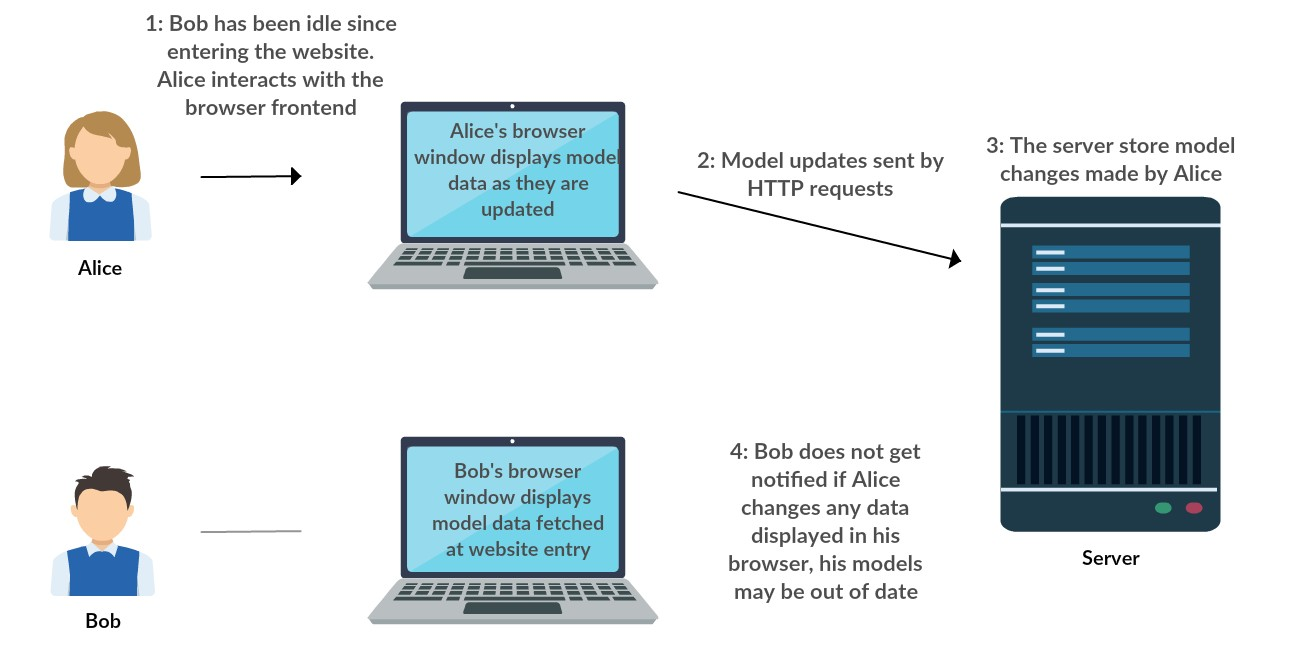
\includegraphics[width=1\textwidth]{figs/update_problem.jpg}
    \caption{Example of updating models without model change notifications}
    \label{fig:update-problem}
\end{figure}

Many websites requires to share data between multiple clients and dynamically notify clients if there are changes to the data. As an example in the \gls{cmb} system, it would be nice if the frontend interface dynamically updated as a user's submission finished running at the backend. In the old system before the improvements, the user had to manually refresh by clicking at a refresh button provided by the user interface or manually refresh the webpage. However, this section presents a technology which has been introduced in the new version of the system in order to dynamically update data relevant for multiple clients. \\

Socket.io \cite{SOCKETIO} is an \gls{api} for enabling real time communication between the server and connected clients. The \gls{api} was first made as Javascript library, but many open source projects have developed modules integrating Socket.io. One benefit of the \gls{api} is that it works as a wrapper around a set of real time communication protocols to enable support for different browsers, which means that the framework can automatically detect the protocol supported by a given browser and use that information to select the best fitted communication protocol. \\

Rohit Rai stated the communication protocols supported by the Socket.io \gls{api} \cite{Rai2013}. Figure \ref{} shows the communication protocols that is enabled in the new version of \gls{cmb}. + figure explaining polling, long polling and websockets. The below sub-sections describes the changes done on the server and frontend code in order to support real time communication with Socket.io\\

\subsection{Server Changes}
The Python module Flask-SocketIO enables the Flask applications access to the SocketIO \gls{api}. To support

\subsection{Frontend Changes}

\section{Server}

\subsection{Database Management System}
SQLAlchemy MYSQL adapter + possible async library.

\subsection{Database Model Updates}
Detailed state field added and can be replaced with json structures as more information is needed about a run.

\subsection{Admin Interface}

Bug fix: Unix vs DOS files.
Cascading delete.

\section{Frontend}
\subsection{Bug Fixes}
Upload fixes in frontend
Sorting bug

\subsection{Views and Feedback}
Spinners + better error messages. Bulletin board to display administrator messages.

\subsection{Group Functionality Improvements}
Moved

\section{Backend}
Some small changes needed to be done at the backend in order to improve the feedback given to the user


\section{Improvement Proposals}
